\documentclass[12pt, twoside]{article}
\usepackage[letterpaper, margin=1in, headsep=0.5in]{geometry}
\usepackage[english]{babel}
\usepackage[utf8]{inputenc}
\usepackage{amsmath}
\usepackage{amsfonts}
\usepackage{amssymb}
\usepackage{tikz}
\usetikzlibrary{quotes, angles}
\usepackage{graphicx}
\usepackage{enumitem}
\usepackage{multicol}
\usepackage{hyperref}

\newif\ifmeta
\metatrue %print standards and topics tags

\title{IB Mathematics}
\author{Chris Huson}
\date{January 2022}

\usepackage{fancyhdr}
\pagestyle{fancy}
\fancyhf{}
\renewcommand{\headrulewidth}{0pt} % disable the underline of the header
\raggedbottom


\fancyhead[LE]{\thepage}
\fancyhead[RO]{\thepage \\ Name: \hspace{4cm} \,\\}
\fancyhead[LO]{BECA / IB Math 03-Quadratic functions\\* 28 January 2022}

\begin{document}

\subsubsection*{4.5 Classwork: Cubic function applications}
\begin{enumerate}
\item Do Now: A function composed of four points $\{ (-1,1),(j,2),(4,1),(5,k) \}$ is plotted on the below.
    \begin{multicols}{2}
    \begin{enumerate}
      \item Write down $j$
      \item Write down $k$
      \item Write down the domain.\vspace{0.5cm}
      \item Add an ordered pair to the relation so that it would \emph{not} be a function. \vspace{1cm}
    \end{enumerate}
      \begin{tikzpicture}[scale=0.8]
        %\draw [help lines] (-3,-2) grid (4,6);
        \draw [thick, ->] (-2.2,0) -- (5.4,0) node [below right] {$x$};
        \draw [thick, ->] (0,-0.5)--(0,5.4) node [left] {$y$};
        \foreach \x in {-2,-1,1,2,..., 5} \draw (\x cm,1pt) -- (\x cm,-1pt) node[anchor=north] {$\x$};
        \foreach \y in {1, 2, 3, 4, 5} \draw (1pt,\y cm) -- (-1pt,\y cm) node[anchor=east] {$\y$};
        %\draw [thick, <->] (-3.5,-1.5) -- (4.2,6.2);
        \fill (-1,1) circle[radius=0.1] node[above left]{$(-1,1)$};
        \fill (2,2) circle[radius=0.1] node[above]{$(j,2)$};
        \fill (4,1) circle[radius=0.1] node[above]{$(4,1)$};
        \fill (5,4) circle[radius=0.1] node[above right]{$(5,k)$};
      \end{tikzpicture}
    \end{multicols}
    
\item The graph of a function $f$ is shown on the grid below.
    \begin{multicols}{2}
    \begin{enumerate}
      \item Write down $f(-2)$
      %\vspace{0.25cm}
      \item Find $x$ for $f(x)=1$.
      \vspace{0.25cm}
      \item Write down the domain.
      \item Write down the range. \vspace{1cm}
    \end{enumerate}
      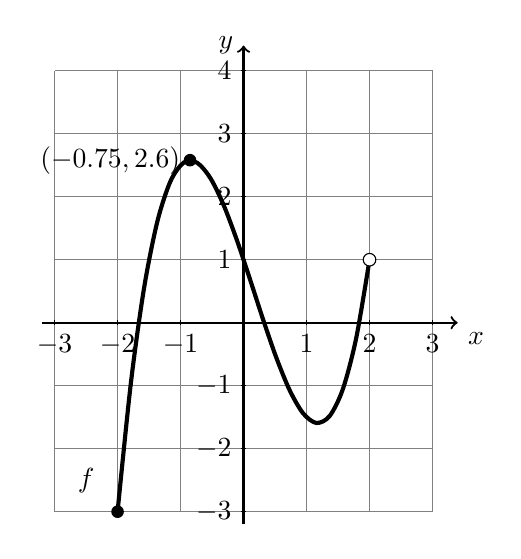
\begin{tikzpicture}[scale=0.8]
        \draw [help lines] (-3,-3) grid (3,4);
        \draw [thick, ->] (-3.2,0) -- (3.4,0) node [below right] {$x$};
        \draw [thick, ->] (0,-3.2)--(0,4.4) node [left] {$y$};
        \foreach \x in {-3,-2,-1,1,2, ...,3} \draw (\x cm,1pt) -- (\x cm,-1pt) node[anchor=north] {$\x$};
        \foreach \y in {-3,-2,-1,1,2,3,4} \draw (1pt,\y cm) -- (-1pt,\y cm) node[left] {$\y$};
        %\draw [thick] (-2,0) -- (0,4) -- (3,5);
        \draw [line width=1.5pt,smooth,samples=20,domain=-2:2] plot(\x,\x^3-0.5*\x*\x-3*\x+1);
        \fill (-2,-3) circle[radius=0.1];
        \fill (-0.85,2.58) circle[radius=0.1] node [left]{$(-0.75,2.6)$};
        \node at (-2.5,-2.5){$f$};
        \fill [white] (2,1) circle[radius=0.1];
        \draw (2,1) circle[radius=0.1];
      \end{tikzpicture}
    \end{multicols}

\item The ramp in a skateboard park is modeled by the cubic function $h(x)=7.25-2.2x+0.011x^{3}$ where $h$ is the height in feet above ground and $x$ is the horizontal distance (ft).
\begin{multicols}{2}
    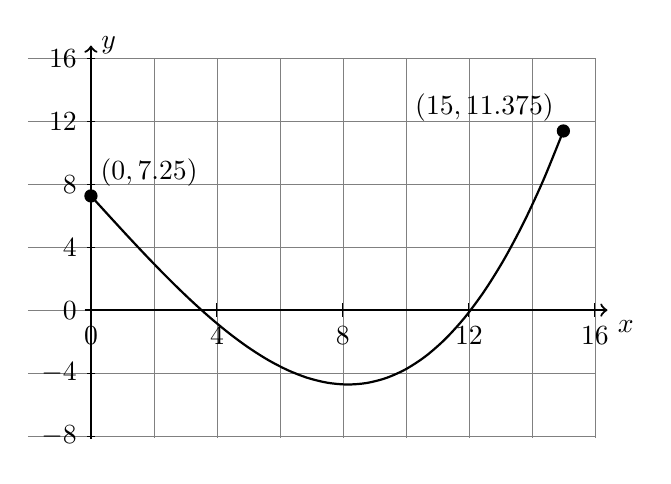
\begin{tikzpicture}[x=0.5cm, y=0.25cm, scale=0.8]
        \draw [help lines] (-2,-8.1) grid (16,16);
        \draw [thick, ->] (-0.2,0) -- (16.4,0) node [below right] {$x$};
        \draw [thick, ->] (0,-8.2)--(0,16.8) node [right] {$y$};
        \foreach \x in {0,4,...,16}
            \draw[shift={(\x,0)}] (0,3pt)--(0,-3pt) node[below] {$\x$};
        \foreach \y in {-8,-4,...,16}
            \draw[shift={(0,\y)}] (2pt,0pt)--(-2pt,0pt) node[left]  {$\y$};
        \draw [-,thick,smooth,domain=0:15] plot(\x,{0.011*(\x)^3+0*(\x)^2-2.2*(\x)+7.25});
        \fill (0,7.25) ellipse(3pt and 3pt) node [above right]{$(0,7.25)$};
        \fill (15,11.375) ellipse(3pt and 3pt) node [above left]{$(15,11.375)$};
    \end{tikzpicture}
\begin{enumerate}[itemsep=0.75cm]
    \item How wide is the ramp in feet?
    \item Which lip is higher, the right or left lip? By how much?
    \item What is the maximum depth below ground of the ramp?
\end{enumerate} 
\end{multicols}

\newpage
\item A cardboard box manufacturing company is building boxes with length represented by $x+1$, width by $5-x$, and height by $x-1$. The volume of the box is modeled by the function below.
\begin{multicols}{2}
    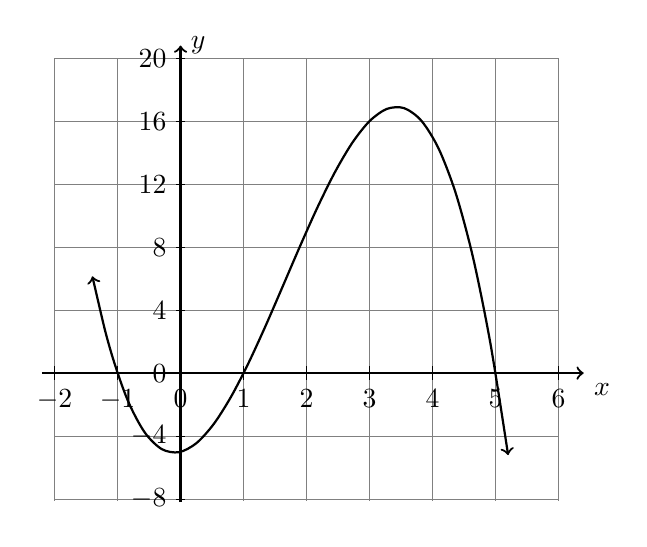
\begin{tikzpicture}[x=1cm, y=0.25cm, scale=0.8]
        \draw [help lines] (-2,-8.1) grid (6,20);
        \draw [thick, ->] (-2.2,0) -- (6.4,0) node [below right] {$x$};
        \draw [thick, ->] (0,-8.2)--(0,20.8) node [right] {$y$};
        \foreach \x in {-2,...,6}
            \draw[shift={(\x,0)}] (0,3pt)--(0,-3pt) node[below] {$\x$};
        \foreach \y in {-8,-4,...,20}
            \draw[shift={(0,\y)}] (2pt,0pt)--(-2pt,0pt) node[left]  {$\y$};
        \draw [<->,thick,smooth,domain=-1.4:5.2] plot(\x,{-(\x)^3+5*(\x)^2+(\x)-5});
    \end{tikzpicture}
\begin{enumerate}[itemsep=0.75cm]
    \item Over what interval of positive $x$ values is the volume positive?
    \item Estimate the maximum possible volume of the box.
    \item Find the value of $x$ would maximize the volume of the box.
\end{enumerate} 
\end{multicols}
%\vspace{0.5cm}

\item Shown in the plot below is the function $f(x)=x^3+4x^2-1x-4$.
\begin{enumerate}
    \item Write down the value of $f(0)$. On the graph, mark the point for $f(0)$ with a star.\vspace{0.75cm}
    \item Write down the solutions to $f(x)=0$. Mark them with ``X'' marks on the graph.\vspace{0.75cm}
    \item Mark the portion of the function that is \emph{decreasing} with a squiggly line.
\end{enumerate}
\begin{center}
    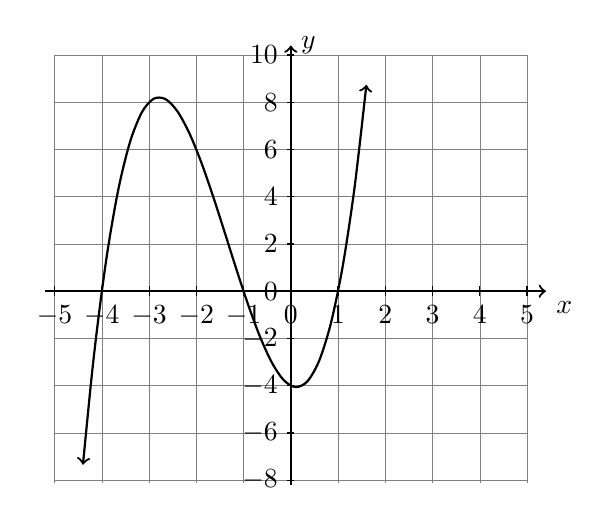
\begin{tikzpicture}[x=1cm, y=0.5cm, scale=0.6]
        \draw [help lines] (-5,-8.1) grid (5,10);
        \draw [thick, ->] (-5.2,0) -- (5.4,0) node [below right] {$x$};
        \draw [thick, ->] (0,-8.2)--(0,10.4) node [right] {$y$};
        \foreach \x in {-5,...,5}
            \draw[shift={(\x,0)}] (0,3pt)--(0,-3pt) node[below] {$\x$};
        \foreach \y in {-8,-6,...,10}
            \draw[shift={(0,\y)}] (2pt,0pt)--(-2pt,0pt) node[left]  {$\y$};
        \draw [<->,thick,smooth,domain=-4.4:1.6] plot(\x,{(\x)^3+4*(\x)^2-(\x)-4});
    \end{tikzpicture}
\end{center}

\end{enumerate}
\end{document}



